\documentclass[12pt]{beamer}
%\documentclass[20pt,handout]{beamer}
\usetheme{Darmstadt}
\usepackage{graphicx}
\usepackage[german]{babel}
\usepackage[T1]{fontenc}
\usepackage[utf8]{inputenc}
\usepackage{tikz}
\setbeamertemplate{footline}[frame number]

\newcommand{\cc}[1]{\includegraphics[height=4mm]{img/#1.png}}
\usepackage{ifthen}
\newcommand{\license}[2][]{\\#2\ifthenelse{\equal{#1}{}}{}{\\\scriptsize\url{#1}}}
\usepackage{textcomp}

\pgfdeclareimage[height=.6cm]{c3d2logo}{./img/c3d2.pdf} 


\pgfdeclarelayer{foreground}
\pgfsetlayers{main,foreground}
\logo{\pgfputat{\pgfxy(-1,0)}{\pgfbox[center,base]{\pgfuseimage{c3d2logo}}}}


\title{Chaos macht Schule}
\author{\small Marius Melzer \& Stephan Thamm\\\large Chaos Computer Club Dresden}
\date{\today}

\begin{document}
\maketitle

\section{Einleitung}

\begin{frame}
  \frametitle{Einleitung}
  \begin{figure}
    
\includegraphics[height=0.7\textheight]{img/fingerabdruck.jpg}
  \end{figure}
\end{frame}

\begin{frame}
  \frametitle{Einleitung}
  \begin{figure}
    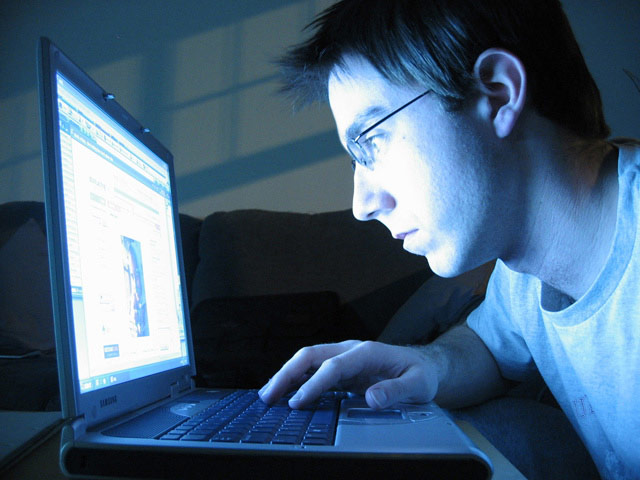
\includegraphics[height=0.7\textheight]{img/internet_user1.jpg}
  \end{figure}
\end{frame}

\begin{frame}
  \frametitle{Einleitung}
  \begin{figure}
    
\includegraphics[height=0.7\textheight]{img/internet_user3.jpg}
  \end{figure}
\end{frame}

\begin{frame}
  \frametitle{Einleitung}
  \begin{figure}
    
\includegraphics[height=0.7\textheight]{img/internet_user4.jpg}
  \end{figure}
\end{frame}

\begin{frame}
  \frametitle{Einleitung}
  \begin{figure}
    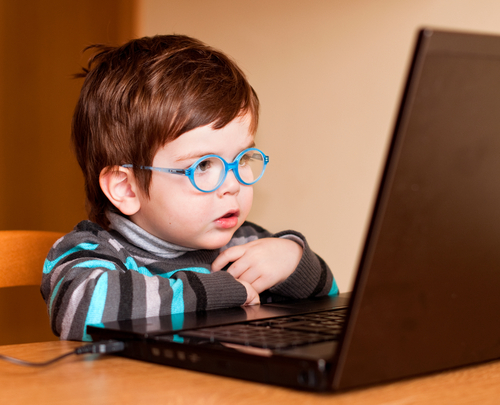
\includegraphics[height=0.7\textheight]{img/internet_user2.jpg}
  \end{figure}
\end{frame}

\begin{frame}
  \frametitle{Gliederung}
  \begin{itemize} \Large
    \item Grundlagen des Internets
    \item Personalisiertes Web
    \item Soziale Netzwerke
    \item Datenschutz
  \end{itemize}
\end{frame}

\section{Grundlagen des Internets}

\begin{frame}
  \frametitle{Grundlagen des Internets}
  \begin{figure}
    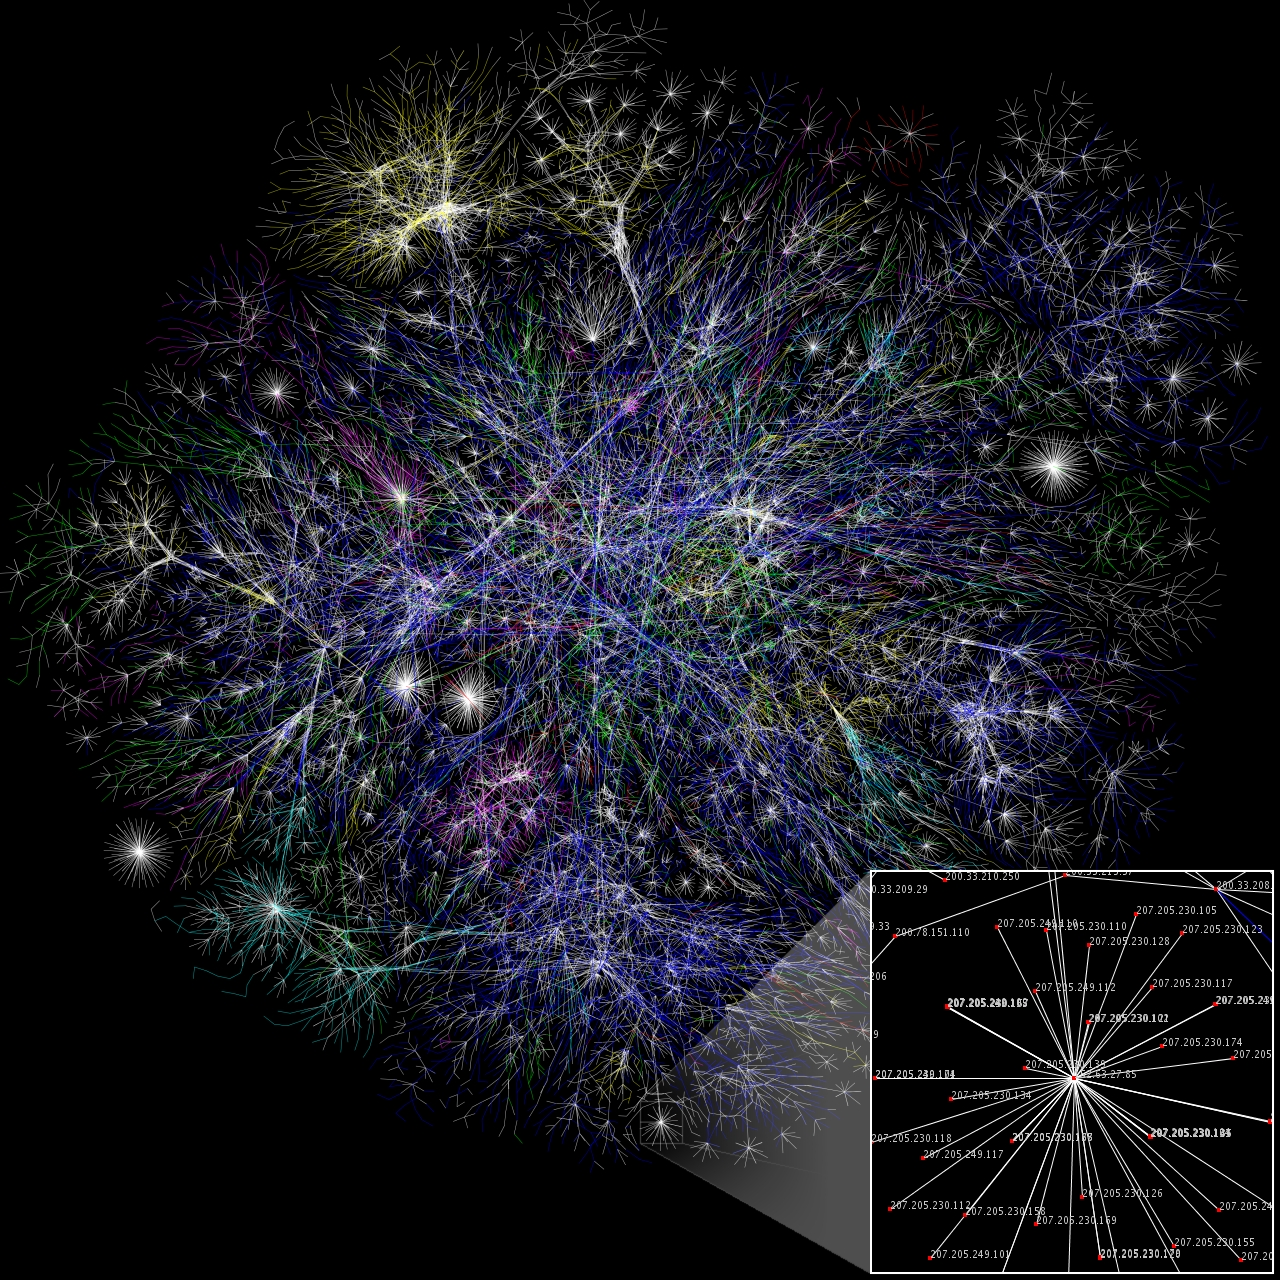
\includegraphics[height=0.7\textheight]{img/internet_map.jpg}
  \end{figure}
\end{frame}

\begin{frame}
  \frametitle{Grundlagen des Internets}
  \begin{center} \Large
    Praxis: Internetgrundlagen
  \end{center}
\end{frame}

\begin{frame}
  \frametitle{Grundlagen des Internets}
  \begin{center} \Large
  DNS
  \end{center}
\end{frame}

\begin{frame}
  \frametitle{Gliederung}
  \begin{itemize}
    \item Vorteile des Internets:
      \begin{itemize}
        \item Soziale Netzwerke
        \item Datenschutz
      \end{itemize}
  \end{itemize}
\end{frame}

\begin{frame}
  \frametitle{Grundlagen des Internets}
  \begin{center} \Large
  Abhören von Netzwerkverkehr
  \end{center}
\end{frame}

\begin{frame}
  \frametitle{Grundlagen des Internets}
  \begin{center} \Large
  Verschlüsselung
  \end{center}
\end{frame}

\section{Personalisiertes Web}

\begin{frame}
  \frametitle{Personalisiertes Web}
  \begin{center} \Large
  Wer?
  \end{center}
\end{frame}

\begin{frame}
  \frametitle{Personalisiertes Web}
  \begin{itemize}
    \item<1-> Wie?
      \begin{itemize}
        \item<2-> Referrer
        \item<3-> Cookies (Demo)
        \item<4-> Zählpixel (Demo)
        \item<5-> Like-Buttons, Facebook-Login, Apps + Spiele
      \end{itemize}
  \end{itemize}
\end{frame}

\begin{frame}
  \frametitle{Personalisiertes Web}
  \begin{itemize}
    \item<1-> Gegenmaßnahmen 
      \begin{itemize}
        \item<2-> Ghostery
        \item<3-> Einstellungen im Browser
        \item<4-> Adblock
      \end{itemize}
  \end{itemize}
\end{frame}

\begin{frame}
  \frametitle{Personalisiertes Web}
  \begin{center} \Large
    https://panopticlick.eff.org/
  \end{center}
\end{frame}

\begin{frame}
  \frametitle{Personalisiertes Web}
  \begin{center} \Large
    Suchmaschinen
  \end{center}
\end{frame}

\begin{frame}
  \frametitle{Personalisiertes Web}
  \begin{center} \Large
     Pseudonymität
  \end{center}
\end{frame}

\begin{frame}
  \frametitle{Personalisiertes Web}
  \begin{itemize}
    \item Passwortsicherheit 
      \begin{itemize}
        \item (nCuAj.§Tsm!f
        \item IchLiebeDich
        \item .§)=")=`
        \item 123456
        \item alkmgfksjr
        \item Mks?o/.u,ePsw!
      \end{itemize}
  \end{itemize}
\end{frame}

\begin{frame}
  \frametitle{Personalisiertes Web}
  \begin{center} \Large
     http://howsecureismypassword.net/
  \end{center}
\end{frame}

\section{Soziale Netzwerke}

\begin{frame}
  \frametitle{Soziale Netzwerke}

  \begin{itemize}
    \item Wer ist in welchem sozialen Netzwerk?
      \begin{itemize}
        \item SchülerVZ
        \item SchülerCC
        \item Facebook
        \item Google+
        \item ICQ/MSN/Jabber
        \item Flickr
        \item Last.fm / Jamendo
        \item Youtube
        \item weitere?
      \end{itemize}
  \end{itemize}
\end{frame}

\begin{frame}
  \frametitle{Soziale Netzwerke}

  \begin{center} \Large
    Praxis: Soziale Netzwerke 
  \end{center}
\end{frame}

\begin{frame}
  \frametitle{Soziale Netzwerke}

  \begin{itemize}
    \item Womit verdienen folgende Firmen ihr Geld?
      \begin{itemize}
        \item<2-> Karstadt
        \item<3-> Amazon
        \item<4-> Ebay
        \item<5-> Facebook
      \end{itemize}
  \end{itemize}
\end{frame}

\begin{frame}
  \frametitle{Einleitung}
  \begin{figure}
    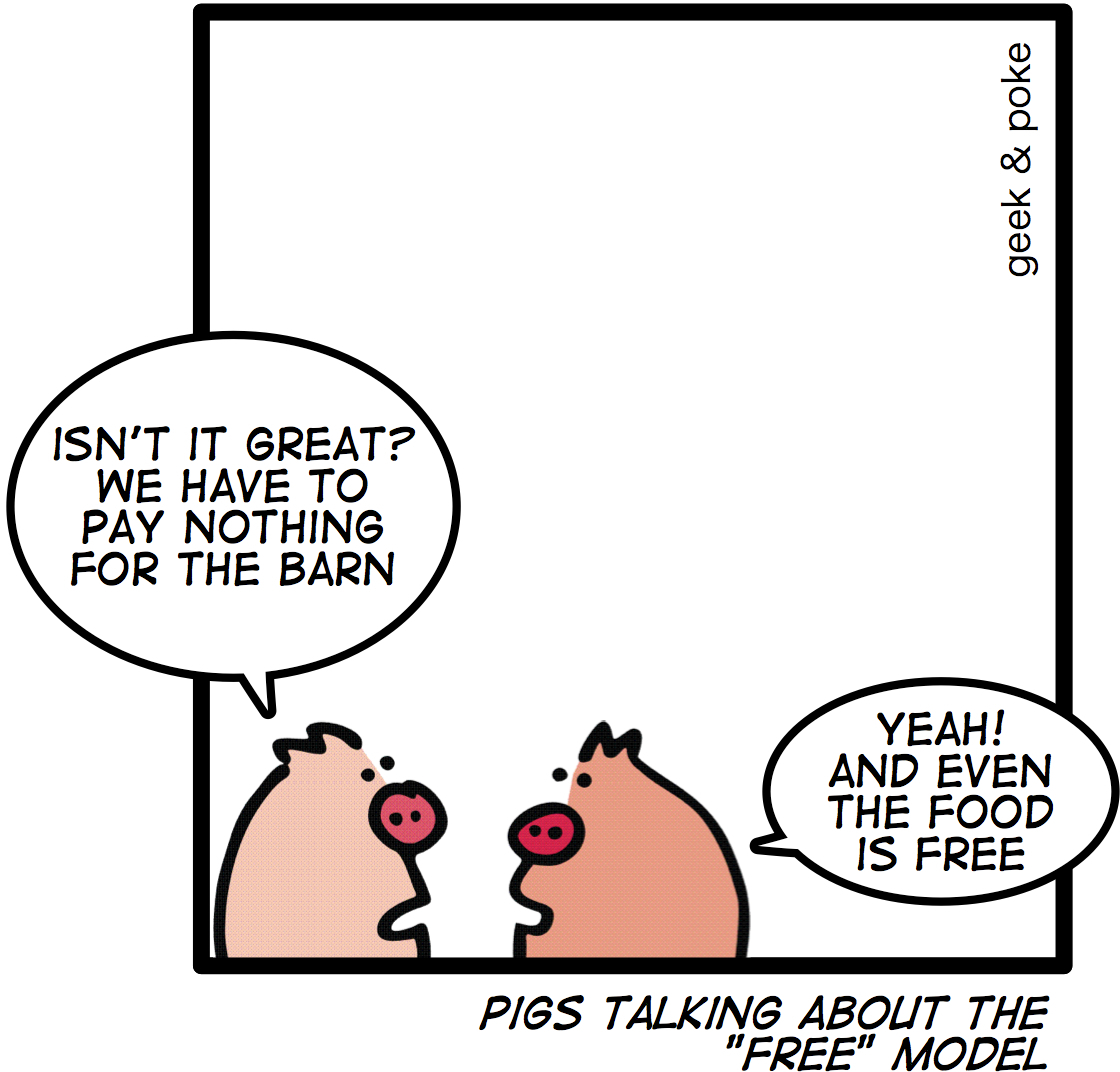
\includegraphics[height=0.7\textheight]{img/business_pigs.jpg}
  \end{figure}
\end{frame}

\begin{frame}
  \frametitle{Soziale Netzwerke}

  \begin{center} \Large
     Was bieten soziale Netzwerke?
  \end{center}
\end{frame}

\begin{frame}
  \frametitle{Soziale Netzwerke}

  \begin{itemize}
    \item Was haben soziale Netzwerke von euch?\\(am Bsp. von Facebook)
      \begin{itemize}
        \item<2-> 82\% Einnahmen aus Werbung
        \item<3-> 30\% Anteil an "`Facebook-Einkäufen"'
        \item<4-> durchschnittlich 1€/Profil
        \item<5-> "`Poweruser"'-Profile deutlich mehr
        \item<6-> => Mehr Werbegewinn durch personalisierte Werbung
      \end{itemize}
  \end{itemize}
\end{frame}

\begin{frame}
  \frametitle{Soziale Netzwerke}

  \begin{itemize}
    \item (Weitere) Probleme
      \begin{itemize}
        \item Datenschutz
        \item Identitätsdiebstahl
      \end{itemize}
  \end{itemize}
\end{frame}

\begin{frame}
  \frametitle{Soziale Netzwerke}

  \begin{center} \Large
    Datenschutz: Einstellungen 
  \end{center}
\end{frame}

\begin{frame}
  \frametitle{Soziale Netzwerke}

  \begin{figure}
    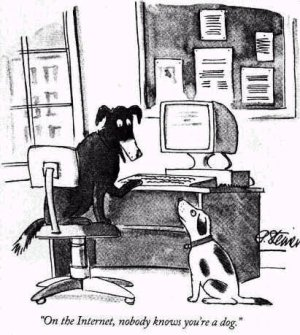
\includegraphics[height=0.7\textheight]{img/internet_dog.jpg}
    \license[http://en.wikipedia.org/wiki/File:Internet\_dog.jpg]{\copyright Image from New Yorker cartoon by Peter Steiner.}
  \end{figure}
\end{frame}

\begin{frame}
  \frametitle{Soziale Netzwerke}

  \begin{center} \Large
    Identitätsklau - aus Sicht des Angreifers
  \end{center}
\end{frame}

\begin{frame}
  \frametitle{Soziale Netzwerke}

  \begin{center} \Large
   Alternativen zu Facebook und co. 
  \end{center}
\end{frame}

\section{Datenschutz}

\begin{frame}
  \frametitle{Datenschutz}

  \begin{center} \Large
   Was ist das und wieso braucht man das? 
  \end{center}
\end{frame}

\begin{frame}
  \frametitle{Datenschutz}

  \begin{itemize}
    \item Wem gegenüber?
      \begin{itemize}
        \item<2-> Eltern
        \item<3-> Lehrern
        \item<4-> Freunden
        \item<5-> Unternehmen / Organisationen
        \item<6-> Staat
      \end{itemize}
  \end{itemize}
\end{frame}

\begin{frame}
  \frametitle{Datenschutz}

  \begin{center} \Large
   Für wieviel Geld würdet ihr eure (Profil-)Daten verkaufen?
  \end{center}
\end{frame}

\begin{frame}
  \frametitle{Datenschutz}

  \begin{itemize}
    \item Wem sollte man preisgeben/posten (und was eher nicht)?
      \begin{itemize}
        \item<2-> "`Roadkill"' von Entertainment for the Braindead ist ein cooles Album
        \item<3-> Jan Müller geht am Donnerstag, den 07.06.2012 zum Poetry Slam in der Scheune
        \item<4-> Ich bin heut' echt gut drauf!
        \item<5-> Ute Meyer war mit Carolin Wittich und Frederik Ulm am Samstag abend im Schillergarten Fußball gucken und ist danach mit Michael Müller nach Hause gefahren
        \item<6-> Meine Lehrerin ist voll doof!
      \end{itemize}
  \end{itemize}
\end{frame}

\begin{frame}
  \frametitle{Datenschutz}

  \begin{center} \Large
   http://www.weknowwhatyouredoing.com/
  \end{center}
\end{frame}

\begin{frame}
  \frametitle{Datenschutz}

  \begin{center} \Large
   Das Internet vergisst nichts!
  \end{center}
\end{frame}

\begin{frame}
  \frametitle{Datenschutz}

  \begin{center} \Large
   Beispiel aus der realen Welt:\\ Schufa und Facebook
  \end{center}
\end{frame}

\begin{frame}
  \frametitle{Datenschutz}

  \begin{center} \Large
   diggr
  \end{center}
\end{frame}

\begin{frame}
  \frametitle{Datenschutz}

  \begin{itemize}
    \item Datenschutz anderer Personen respektieren:
      \begin{itemize}
        \item<2->Bilder taggen
        \item<3->Emailadressen importieren
        \item<4->Angeben, mit wem man etwas unternimmt
      \end{itemize}
  \end{itemize}
\end{frame}

\begin{frame}
  \frametitle{Datenschutz}

  \begin{itemize}
    \item Eigenschutz
      \begin{itemize}
        \item<2->Moderation von Posts
        \item<3->Freunde auf Fehlverhalten hinweisen
        \item<4->Aufpassen was und wieviel man preisgiebt
      \end{itemize}
  \end{itemize}
\end{frame}

\end{document}
